\documentclass[emulatestandardclasses]{scrartcl}
\usepackage{graphicx}
\usepackage{color}
\usepackage[ngerman]{babel}
\usepackage{hyperref}
\usepackage{fullpage}
\usepackage{calc} 
\usepackage{enumitem}
\usepackage{titlesec}
\newcommand{\todo}[1]{\textcolor{red}{TODO: #1}\PackageWarning{TODO:}{#1!}}
\date{\vspace{-3ex}}
\begin{document}

\title{
	\includegraphics*[width=0.75\textwidth]{ErstesSem/images/hu_logo.png}\\
	\vspace{24pt}
	Aristoteles\\Nikomachische Ethik}
\subtitle{VEV SS 17\\
          Dr. Philipp Br"ullmann\\
          Philosophische Fakult"at I \\ 
          Humboldt Universit"at zu Berlin}
\author{Lennard Wolf\\
        \small{\href{mailto:lennard.wolf@student.hu-berlin.de}{lennard.wolf@student.hu-berlin.de}}}
\maketitle
\begin{abstract}

Die Nikomachische Ethik des Aristoteles ist eine der interessantesten, einflussreichsten und meistdiskutierten Schriften zur praktischen Philosophie. Sie behandelt eine Vielzahl wichtiger Themen (wie etwa das gute Leben, Tugend, Verantwortung, Gerechtigkeit, Freundschaft, Willensschw"ache, Lust und Erziehung) und entwirft eine Konzeption der Ethik, die systematisch ernstzunehmen ist. Wer sich f"ur praktische Philosophie interessiert, sollte die Nikomachische Ethik kennen. In unserer Vorlesung werden wir uns (a) einen "uberblick "uber die zentralen Thesen und Argumente der Schrift verschaffen und dabei (b) einige Interpretationsprobleme und Forschungskontroversen kennenlernen. Außerdem werden wir (c) versuchen, die Nikomachische Ethik in ihren Kontext, d.h. den Kontext der antiken Ethik und der Aristotelischen Philosophie, einzuordnen und nicht zuletzt (d) immer wieder die Frage stellen, wie sich der Ansatz des Aristoteles zu anderen Ans"atzen in der normativen Ethik verh"alt.
\end{abstract}
\newpage

\tableofcontents
\listoffigures
\newpage


\section{Die Frage nach dem Gl"uck [I 1-5]\\(25.04.17)}

\subsection{Zusammenfassung erste Sitzung}

\begin{itemize}
  \item Unterscheidung Esoterisch/Exoterisch : Ver"offentlicht/Vorlesungen
  \item "`Gl"uck"': objektiv, kontingent
  \item "`Tugend"': technische Definition
  \item Ziel: Tugendhaft zu \emph{werden}, nicht blo"s Theorie kennen
  \item Enger Zusammenhang zwischen Tugend und Gl"uck
  \item Ethik hat hier nichts mit Moral zu tun
\end{itemize}

\noindent \textbf{Ziel der Sitzung:} Wie ist die Frage nach dem Gl"uck formuliert/wie ist das Problem beschrieben?

\subsection{\emph{eudaimonia}}

\begin{description}[leftmargin=!,labelwidth=\widthof{\bfseries Frage nach dem Gl"uck}]
  \item[Frage nach dem Gl"uck] Welches ist das beste Leben, das man f"uhren kann?
\end{description}


\subsection{Die Herausforderung des Amoralisten}

\begin{itemize}
  \item Frage nach dem guten Leben kam schon in Platons fr"uhen Dialogen vor (Sokrates)
  \item Sokrates versucht zu zeigen, dass der Gerechte ein besseres Leben hat als der Ungerechte (es ist f"ur \emph{ihn} besser, gerecht zu sein).
  \item Problem: intuitiv ist ungerecht sein doch von Vorteil f"ur einen
  \item Hirte Gyges (\emph{Politeia}): Ring kann unsichtbar machen, Hirte findet und kann heimlich Unrecht tun. "`W"urden wir das nicht auch alle machen?"'
  \item Herausforderung des Amoralisten: Warum sollen wir dann "uberhaupt gerecht sein?
  \item Genauer: einziger Vorteil eines gerechten Lebens ist Sicherheit vor Strafe
  \item Antwort von Sokrates: Gerechtigkeit ist ein bestimmter Zustand der Seele. Der Ungerechte schadet seiner Seele, er ist quasi \emph{krank}. (Unordnung in der Seele, die Teile der Seele tun nicht das wof"ur sie da sind)
\end{itemize}

\subsection{Aristoteles und der Amoralist}

\begin{itemize}
  \item Aufgabe: Zeigen, dass auch konsequent eigeninteressierte Menschen einen Grund haben, gerecht zu sein
  \item Aristoteles wendet sich nicht an den Amoralisten
  \item Eignet sich nicht f"ur Menschen, die sich nicht von ihren Leidenschaften bestimmen lassen, sowie sittenhaft und gut erzogen sind ($\rightarrow$ gemeinsame Grundlage)
  \item $\rightarrow$ was hei"st das f"ur die Moralpsychologie/das Begr"undungsprojekt?
\end{itemize}

\subsection{Die Frage nach dem Gl"uck}

\subsubsection{Das Anerkannte und das Umstrittene [I 2-3]}

\begin{itemize}
  \item Aristoteles fragt sich: Wor"uber besteht Einigkeit/Uneinigkeit?
  \item \textbf{Uneinigkeit}: Was ist das Gl"uck? | Vielfalt und Relativit"at der Antworten | Lebensformen... Lust (Menge): sklavenartig; Ehre (Politiker): abh"angig von anderen; Gutheit: w"are mit Unt"atigkeit vereinbar; Betrachtung (theoria): ???; Gelderwerb: Mittel zum Zweck
  \item \textbf{Einigkeit}: Das Gl"uck ist das h"ochste durch Handeln erreichbaren G"uter (gut leben, handeln; sich wohl befinden)
  \item Diese Unterscheidung ist Grundlage f"ur Frage: Was ist das h"ochste Gut?
\end{itemize}

\subsubsection{G"uter und Ziele [I 1]}

\begin{itemize}
  \item Kede Kunst, Lehre, Handlung und Entschluss scheint irgendein Gut zu erstreben.
  \item G"uter sind Ziele
  \item Wenn $a$ das Ziel der T"atigkeit $b$ ist, dann ist $a$ "`besser"' (ein h"oheres Gut) als $b$. | Wenn $a$ ein Ziel ist, das wir umwillen eines h"ohren Ziels $b$ ist, dann ist $b$ "`besser"' (ein h"oheres Gut) als $a$.  | (G"uter k"onnen verglichen werden)
  \item H"ochstes Gut: Etwas das wir immer um seiner selbst willen und nie um einer anderen Sache willen erstreben und um dessentwillen wir alles andere erstreben
  \item Die \emph{eudaimonia} ist solch ein h"ochstes Gut
\end{itemize}

\subsubsection{Es gibt keine Idee des Guten [I 4]}

\begin{itemize}
  \item Begriff des h"ochsten Guts in Verkn"upfung mit Platons Ideenlehre: Gegenstand der \emph{gut} im "`h"ochsten Ma"se"' aufweist
  \item $\rightarrow$ Gradueller Unterschied (im Kontrast zu [I 1])
  \item Aristoteles weist diesen Ansatz zur"uck, da G"uter zu verschieden sind; Kennen des abstrakten Guten hilft nichts f"ur den Erwerb der einzelnen, konkreten G"uter
  \item $\rightarrow$ \emph{Nicht hintergehbare Verschiedenheit der G"uter}. Die Ethik muss dieser Verschiedenheit gerecht werden.
\end{itemize}

\subsubsection{Die drei Kriterien [I 5]}

\noindent \textbf{Kriterien die die eudaimonia als h"ochstes Gut auszeichnen:}

\begin{enumerate}
  \item Wir w"ahlen alles um des guten Lebens willen, aber niemals das gute Leben um einer anderen Sache willen.
  \item Die \emph{eudaimonia} ist "`autark"', d.h. wenn wir sie besitzen, dann bed"urfen wir keiner weiteren Dinge (betrifft auch andere Menschen).
  \item Die \emph{eudaimonia} l"asst sich nicht durch die Hinzuf"ugung weiterer G"uter verbessern.
\end{enumerate}

\noindent $\rightarrow$ Vorrauss"atzungen f"ur [I 6 ff.] eine eigene Bestimmung des Gl"ucks zu entwickeln

\subsection{Begriffe}

\begin{description}[leftmargin=!,labelwidth=\widthof{\bfseries \emph{eudaemonia}}]
  \item[\emph{eudaimonia}] \emph{Nicht}: Gl"ucksgef"uhl, oder Zufallsgl"uck | \emph{Sondern}: Ein insgesamt gelungenes Leben | W"ortlich: Unter "`gutem daimon"', unter einem guten Stern stehen (auch: \emph{Gl"uckseligkeit})
    \item[\emph{ergon}] Ergebnis einer T"atigkeit
  \item[\emph{energeia}] Aktualit"at
  \item[\emph{dynamis}] M"oglichkeit/Potenzial
\end{description}

\subsection{Tutorium}

Wir verwenden die  griechischen Ausdr"ucke

\newpage
\section{"Uber den Professor}
Prof. Mustermann ist..


%\begin{figure}[h]
%	\centering
%	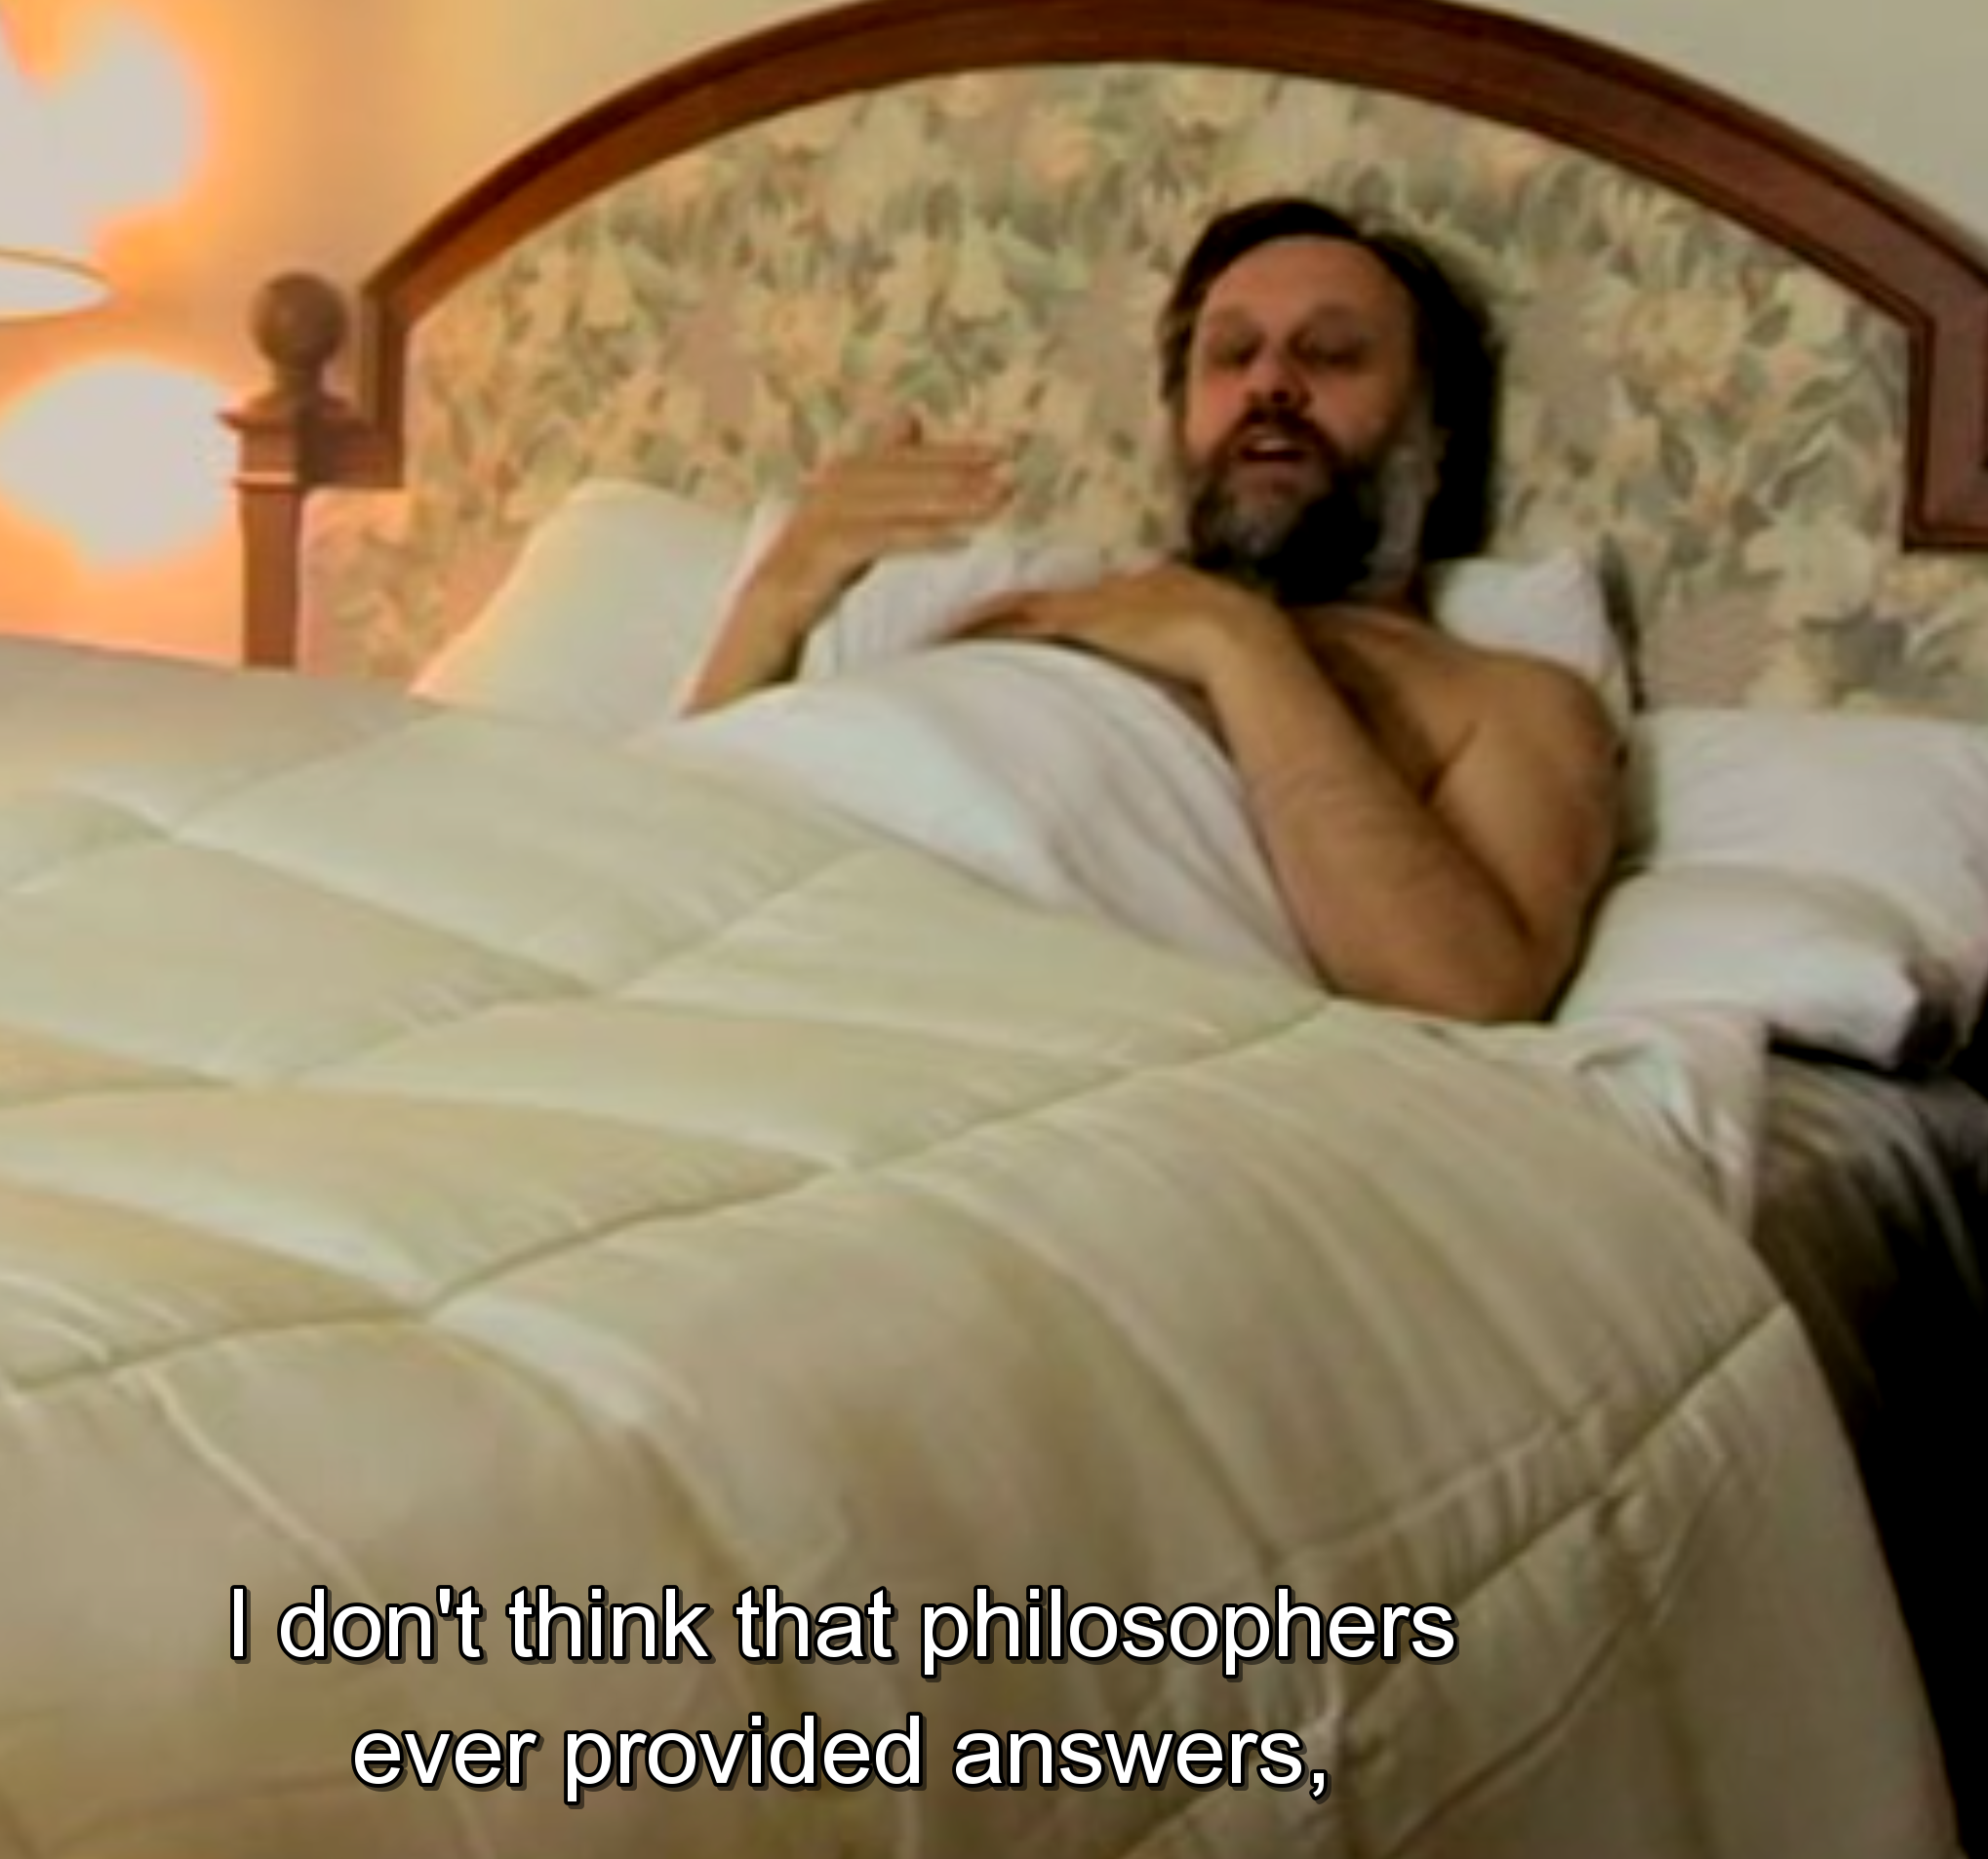
\includegraphics[width=0.5\textwidth]{images/template.png}
%	\caption{Template Bild}
%	\label{fig:template}
%\end{figure}

\end{document}
